\documentclass{pirategame}

% Set the background image
\setBackground{img/paper.jpg}

\begin{document}

% Title Page
\begin{titlepage}
    \centering
    \vspace*{0.5in}
    {\Huge \textbf{Légendes des Caraïbes : le Duel}}\\

    \vspace{0.5in}
    \addLogoWithGradient[1]{img/logo-2.png}\\[1cm]
    \vspace{0.5in}
    {\Large Une expérience immersive pour les passionnés d'airsoft}
    {\large \url{https://leroilion.github.io/airsoft---legende-des-caraibes-le-duel/}}
\end{titlepage}
% \newpage

% Content
\section{Introduction}
\textbf{Bienvenue à bord, moussaillons !} \\
Dans cet âge d'or des pirates, chaque équipage doit prouver sa valeur en partant à la chasse au trésor. Votre mission : parcourir les eaux dangereuses et récupérer un maximum de trésors dissimulés sur l'île. Mais prenez garde, car l'équipage adverse ne reculera devant rien pour vous voler votre butin.

\section{Déroulement de la partie}

\begin{minipage}[t]{0.28\textwidth}
  \vspace{0em}
  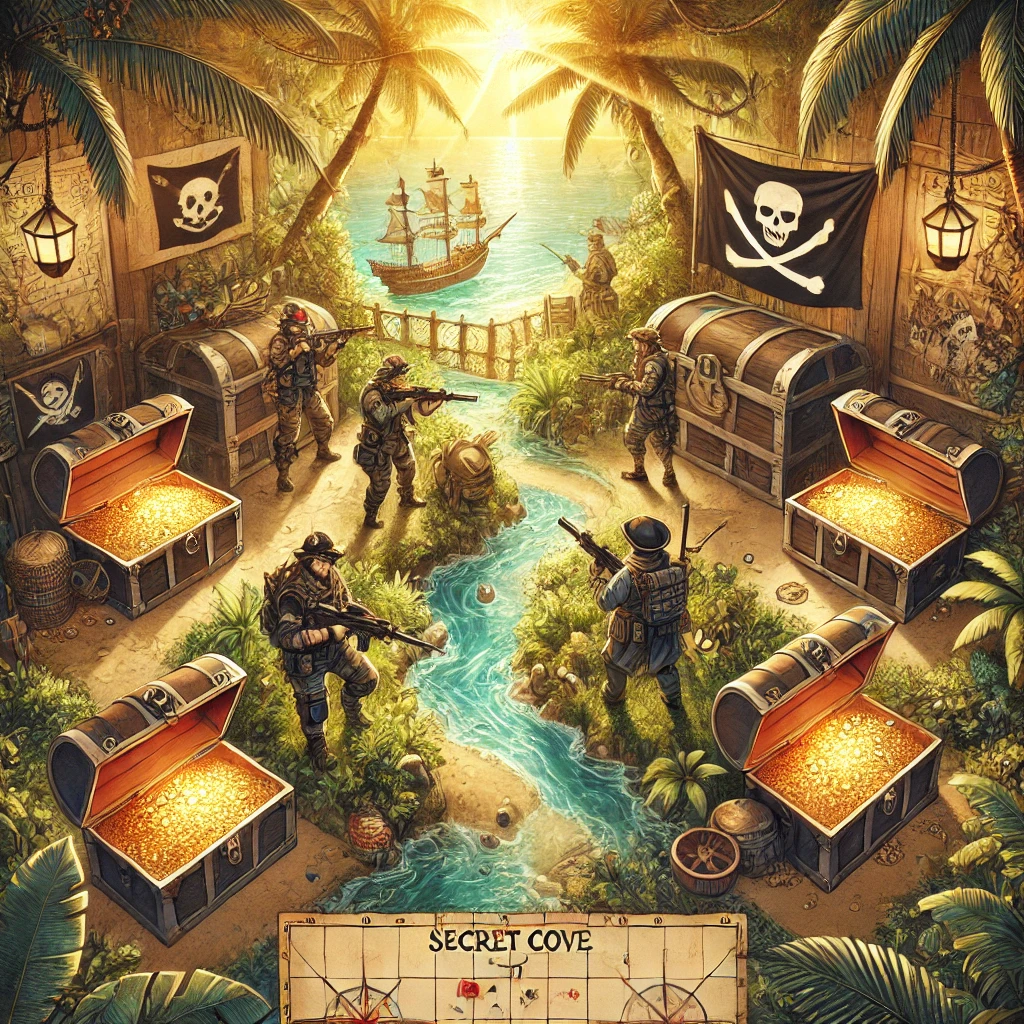
\includegraphics[width=\linewidth]{img/start.png}
\end{minipage}
\hfill
\begin{minipage}[t]{0.7\textwidth}
  Chaque équipage commence dans sa crique secrète, son port d'attache, où se trouve son coffre principal. Vous devrez explorer l'île, repérer les caches au trésor, et ramener votre butin en sécurité dans votre coffre.

  \textbf{Rappelez-vous, pirates :}
  \begin{itemize}
      \item Chaque trésor a une valeur différente. Une pièce d'or ne vaut pas une gemme rare.
      \item Tant que votre trésor n'est pas dans votre coffre, il peut être pillé par vos ennemis !
  \end{itemize}
  
  À la fin de l'aventure, l'équipage ayant accumulé le plus de richesses sera couronné roi des pirates.
\end{minipage}



\section{Fin de la partie}
L'aventure prend fin lorsque :
\begin{itemize}
    \item Le sablier est écoulé (fin du temps imparti).
    \item Tous les trésors ont été découverts et ramenés à bon port.
\end{itemize}

\section{Zones de jeu}
Le terrain représente une île divisée en trois grandes zones :
\begin{itemize}
    \item Une crique secrète pour chaque équipage (zone de départ et de respawn).
    \item La jungle centrale, un terrain dangereux regorgeant de trésors.
\end{itemize}

Les trésors les plus précieux se trouvent dans la jungle, à mi-chemin entre les deux criques. Prenez garde, c'est aussi là que les embuscades sont les plus fréquentes !

\section{Les trésors}

Sur cette île mystérieuse, les trésors prennent diverses formes et ont des valeurs variées :

\begin{minipage}[t]{0.7\textwidth}
  \begin{itemize}[series=treasures]
      \item Une pièce d'argent : valeur 1.
      \item Une pièce d'or : valeur 2.
      \item Une gemme rare : valeur 5.
      \item Une statuette ancienne : valeur 10.
      \item Un masque en or maudit : valeur 10.
  \end{itemize}
\end{minipage}
\hfill
\begin{minipage}[t]{0.28\textwidth}
  \vspace{0em}
  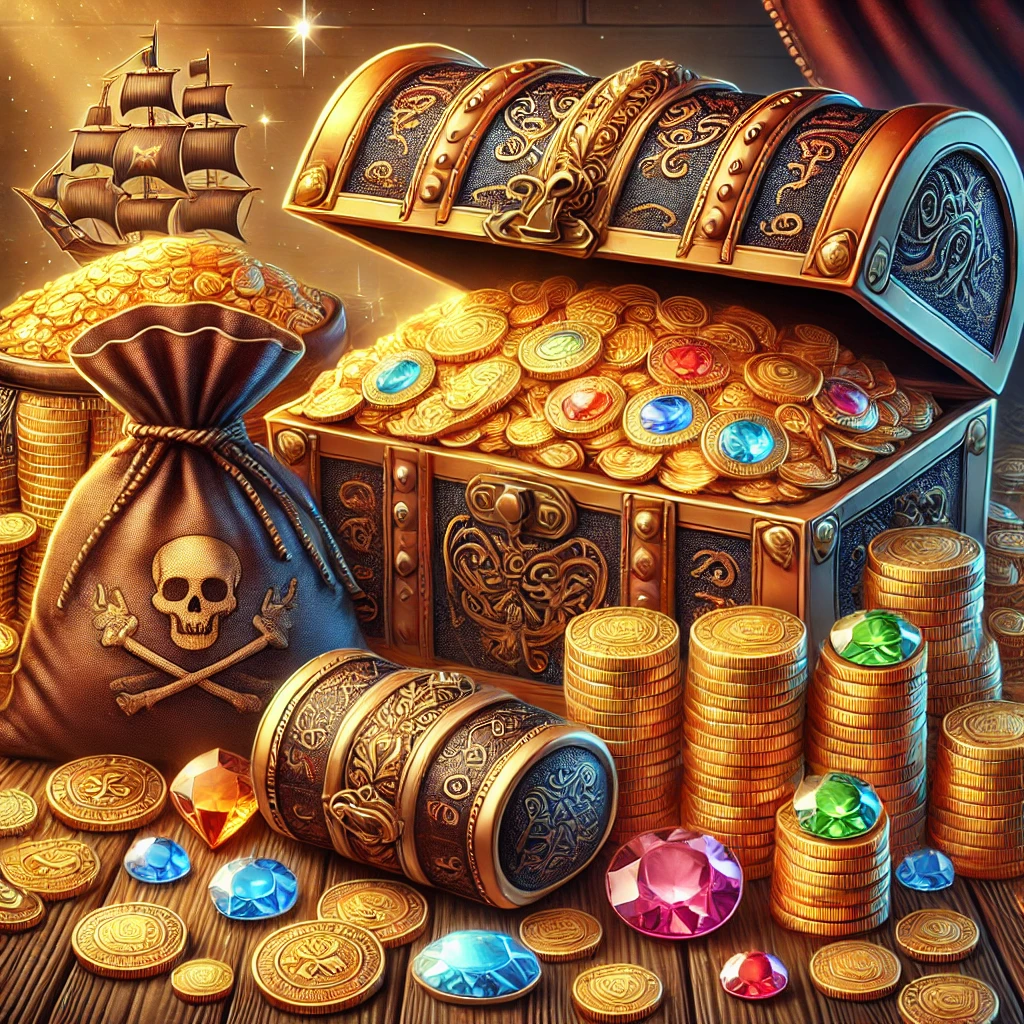
\includegraphics[width=\linewidth]{img/tresors.png}
\end{minipage}


\begin{itemize}[resume*=treasures]
  \item Une bourse de pièces (contenant un nombre aléatoire de pièces).
  \item Un coffre au trésor (renfermant un butin mystérieux : pièces et gemmes rares).
\end{itemize}

\textbf{Attention, pirates :} Les coffres les plus visibles cachent souvent des surprises. Vous ne connaîtrez jamais leur véritable valeur avant de les ouvrir. Prenez des décisions stratégiques, mais rappelez-vous que la cupidité peut vous perdre !



\section{Règles du jeu}

\begin{minipage}[t]{0.7\textwidth}
  \columnsep=0.1\textwidth
  \begin{enumerate}[(1),series=rules]
      \item \textbf{Butin limité :} Un pirate ne peut transporter qu’un seul trésor à la fois.
      \item \textbf{Visibilité du butin :} Un trésor doit toujours être visible et porté à la main. Pas question de le cacher sous votre manteau !
      \item \textbf{Main occupée :} Un pirate tenant un trésor ne peut pas utiliser la main qui le tient pour manier son sabre ou son pistolet.
      \item \textbf{Pas de course effrénée :} Un pirate portant un trésor ne peut pas courir. Une marche rapide, oui, mais pas plus !
  \end{enumerate}
\end{minipage}
\hfill
\begin{minipage}[t]{0.28\textwidth}
  \vspace{0em}
  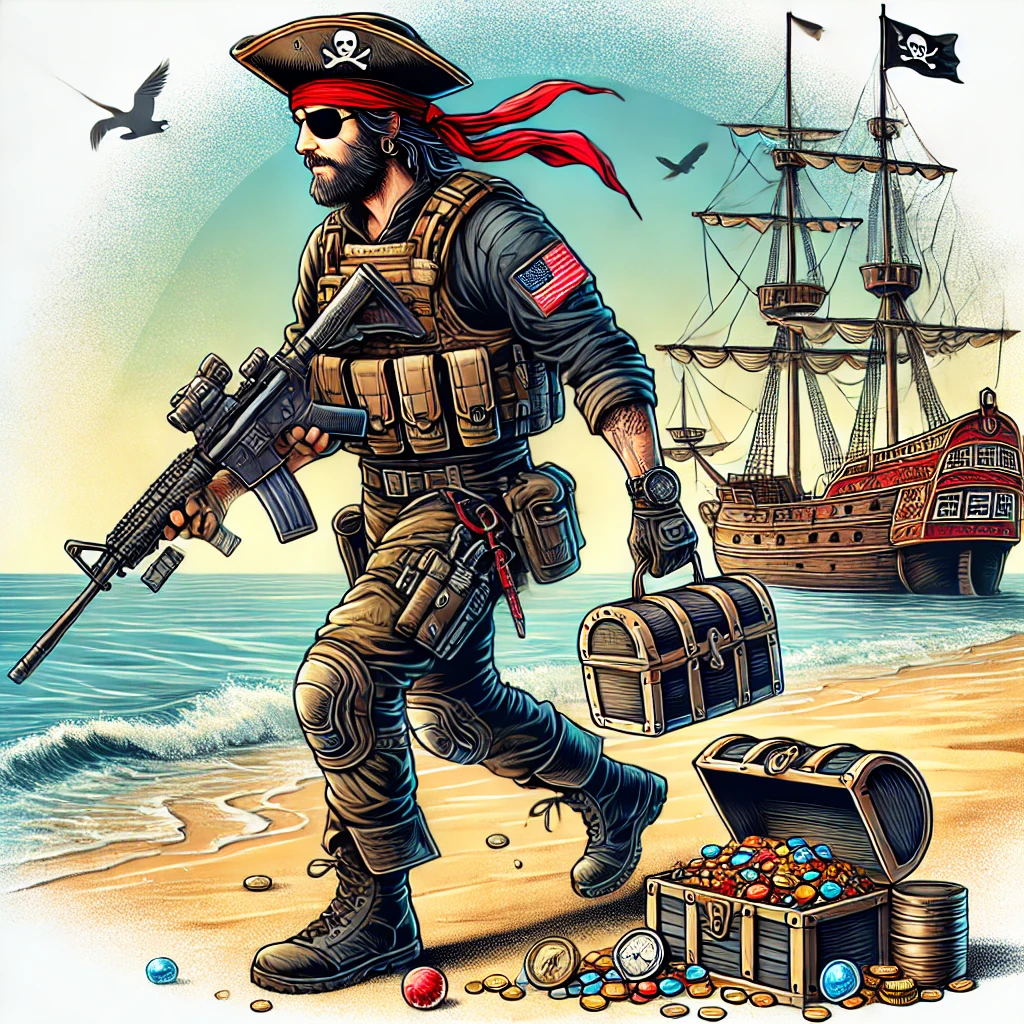
\includegraphics[width=\linewidth]{img/rules-1-2-3-4.png}
\end{minipage}

\begin{enumerate}[resume*=rules]
  \item \textbf{Pose stratégique :} Vous pouvez poser un trésor pour esquiver un ennemi ou vous abriter. Mais attention : tout trésor abandonné devient une proie facile.
  \item \textbf{Échange malin :} Vous pouvez échanger un trésor pour un autre de plus grande valeur, à condition de poser le premier.
  \item \textbf{Trésor touché, pirate maudit :} Si un trésor qu’un pirate transporte est touché par un tir, le pirate est considéré comme atteint par une malédiction et doit immédiatement se déclarer hors jeu
  \item \textbf{Retour après une blessure :} Si vous êtes touché, deux choix s'offrent à vous :
  \begin{itemize}
    \item \textbf{Soins sur le terrain :} Trouvez un camarade médic pour soigner vos blessures pendant que 10 grains s’écoulent dans le sablier (10 secondes). Un pirate ne peut être soigné qu’une seule fois avant de devoir retourner à sa crique.
    \item \textbf{Repos à la crique :} Retournez à votre crique et reposez-vous jusqu’à ce que 30 grains s’écoulent dans le sablier (30 secondes). Une fois reposé, vous pourrez à nouveau recevoir un soin sur le terrain.
  \end{itemize}
\end{enumerate}

\begin{minipage}[t]{0.28\textwidth}
  \vspace{0em}
  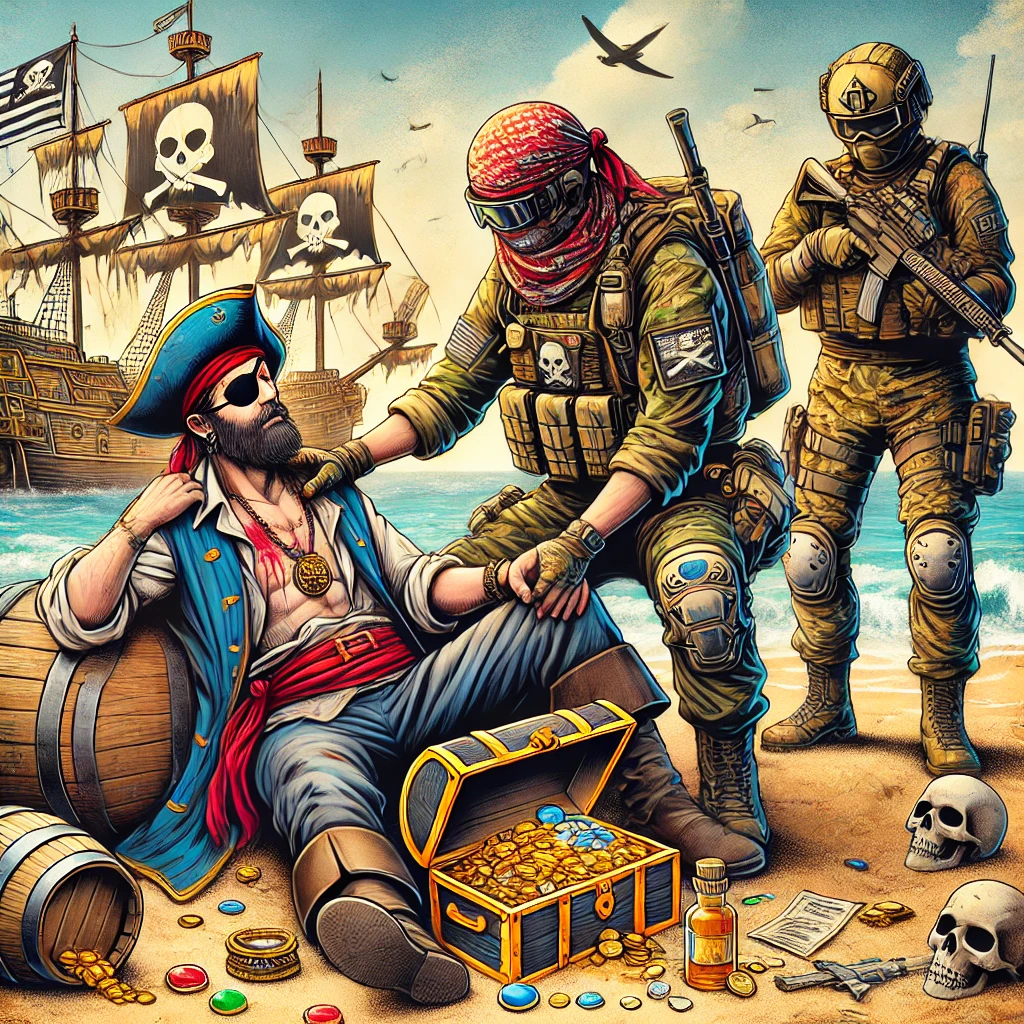
\includegraphics[width=\linewidth]{img/rule-8.png}
\end{minipage}
\hfill
\begin{minipage}[t]{0.7\textwidth}
  \columnsep=0.1\textwidth
  \begin{enumerate}[resume*=rules]
    \item \textbf{Trésor abandonné :} Un pirate blessé doit poser son trésor sur le sol. Il pourra être récupéré par un autre pirate... ou un adversaire !
    \item \textbf{Interdiction de pillage complet, mais observation permise :} Il est interdit de vider un coffre ou une bourse de son contenu. Cependant, un pirate peut jeter un œil furtif pour en évaluer la richesse sans rien déranger.
    \item \textbf{Camouflage et ruses :} Vous pouvez déplacer un trésor ou l'utiliser comme leurre pour tendre un piège. Faites preuve d'ingéniosité !
    \item \textbf{Interdiction de jeter le butin :} Un vrai pirate respecte son trésor ! Il est strictement interdit de lancer un trésor, sous peine de déclencher la colère des esprits marins.
  \end{enumerate}
\end{minipage}

\begin{enumerate}[resume*=rules]
  \item \textbf{Restrictions pour les médecins de bord :}
    \begin{itemize}
      \item Un médecin touché pendant un soin doit se déclarer. Le blessé reste sans soins.
      \item Un médecin ne peut pas manier d'arme pendant qu'il soigne un pirate.
      \item Le médecin doit poser ses deux mains sur le blessé pour canaliser son énergie et lui permettre de revenir au combat.
      \item Le médecin peut déplacer un blessé d'un pas pour le mettre à l’abri.
    \end{itemize}
  \item \textbf{Trésors protégés :} Les coffres des adversaires sont hors limites. Tout pirate enfreignant cette règle sera banni !
  \item \textbf{Retour illimité :} Les pirates ont des vies illimitées, mais doivent respecter les règles de reprise.
  \item \textbf{Respect des coffres :} Tout coffre ouvert doit être refermé. Si vous êtes touché pendant l’action, déclarez-vous et terminez de refermer le coffre.
  \item \textbf{Vérification finale :} À la fin de la partie, chaque pirate est encouragé à vérifier les emplacements où il a déposé des trésors pour aider à leur récupération.
  \item \textbf{Annonce :} Lorsqu'un pirate est touché, il doit le signaler haut et fort en criant "OUT". Lorsqu'il reprend la chasse au trésor, il doit le signaler en criant "REPRISE".
  \item \textbf{Fairplay :} Comme dans toutes les parties d'airsoft, le fairplay de chaque joueur est essentiel pour garantir une expérience agréable pour tous.
  \item \textbf{Prenez du plaisir et amusez-vous !}
\end{enumerate}


\section{Stratégies possibles}
Voici quelques idées pour dominer l'aventure :
\begin{itemize}
  \item Collecter un maximum de petits trésors pour accumuler des points rapidement.
  \item Viser les trésors de grande valeur, même au risque de perdre plus de temps.
  \item Laisser vos ennemis chercher les trésors et leur tendre une embuscade avant qu'ils n'atteignent leur coffre.
  \item Vider un coffre et le laisser vide pour tromper vos adversaires.
  \item Placer une gemme à un endroit exposé pour forcer l’ennemi à se mettre en danger.
  \item Répartir les trésors entre plusieurs membres de l’équipage pour limiter les pertes, ou les confier à un seul pirate pour sécuriser rapidement un gros butin.
\end{itemize}


\section{Suggestion de répartition des trésors}


\subsection{Répartition sur le terrain}

\begin{minipage}[t]{0.7\textwidth}
  % Colonne 1 : Énumération sur 70% de la largeur
  \columnsep=0.1\textwidth % Espacement entre colonnes (facultatif)
  \begin{itemize}[series=repartition]
    \item Vous pouvez ajouter des leurres pour tromper les pirates téméraires (par exemple, des coffres contenant une carte sans trésor ou des bourses remplies de cailloux).
    \item Installez quelques trésors de faible valeur près des zones de départ pour donner un avantage stratégique aux équipages dès le début de l’aventure.
    \item Placez les trésors de grande valeur au centre de l’île, à mi-chemin entre les deux criques secrètes, pour encourager des confrontations épiques.
  \end{itemize}
\end{minipage}
\hfill
\begin{minipage}[t]{0.28\textwidth}
  \vspace{0em}
  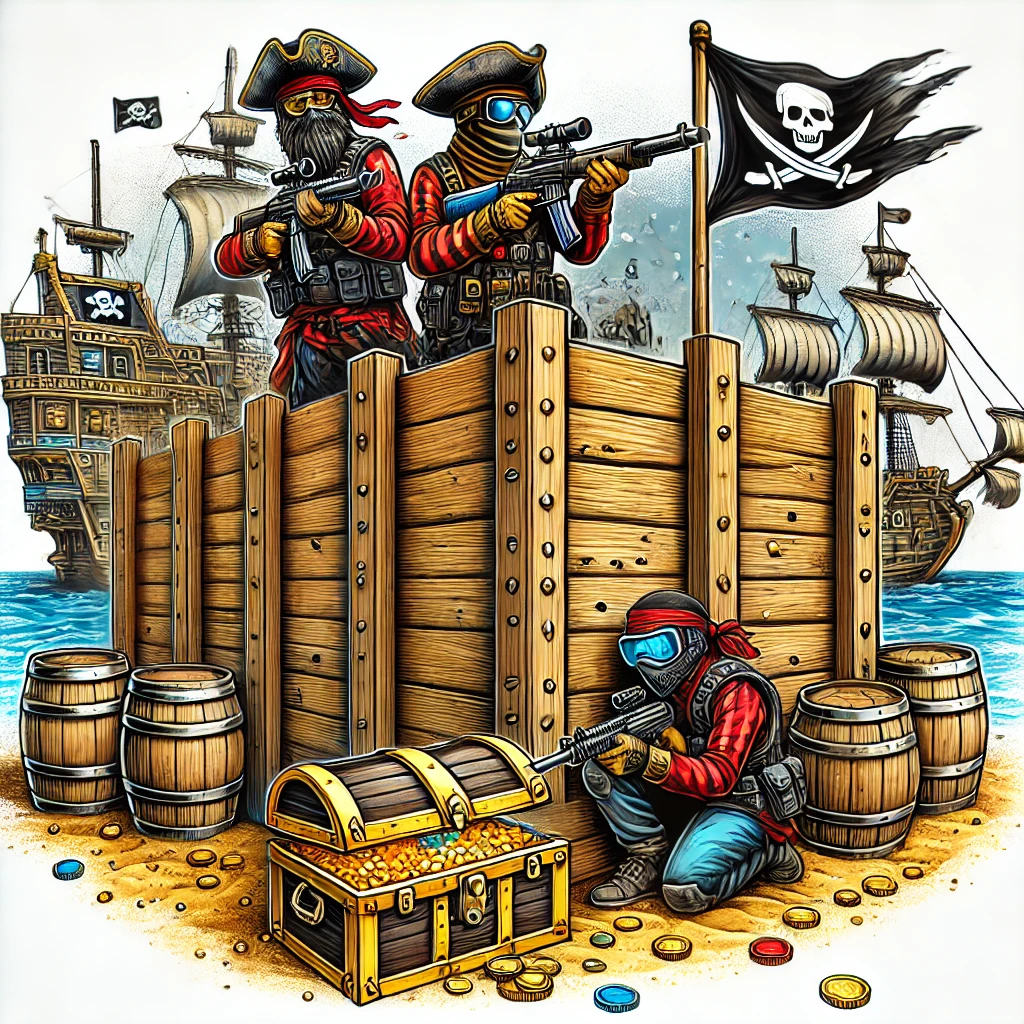
\includegraphics[width=\linewidth]{img/orga-planque-tresor.png}
\end{minipage}

\begin{itemize}[resume*=repartition]
  \item Les trésors peuvent être disposés de manière variée pour enrichir le jeu :
  \begin{itemize}
      \item Cachés au sol, à l’abri des regards indiscrets ;
      \item Bien visibles, pour inciter les pirates à s’aventurer hors de leur cachette ;
      \item Placés en hauteur, proches d’une crique mais facilement défendables par l’équipage adverse, ces trésors forcent les pirates à s’engager dans des manœuvres audacieuses pour les récupérer.
  \end{itemize}
\end{itemize}

\subsection{Exemple de calcul du nombre de trésors et de leur valeur}

Cet exemple est fourni à titre indicatif pour expliquer comment calculer les éléments de jeu à partir de paramètres définis.\\ 
Vous pouvez aussi utiliser le générateur en ligne : \url{https://leroilion.github.io/airsoft---legende-des-caraibes-le-duel/repartition.html}.

\begin{itemize}
  \item \textbf{Définir les paramètres :} Indiquez le nombre de joueurs, la taille des squads dans les deux grandes équipes, et le nombre de trésors à trouver par squad.  
  \textit{Exemple : 40 joueurs, squads de 4 joueurs, et 2 trésors à trouver par squad.}

  \item \textbf{Définir les types et valeurs des trésors :}  
  \textit{Exemple : des pièces (valeur 1), des gemmes (valeur 2), 2 statuettes, et un masque en or.}

  \item \textbf{Définir la répartition bourses / coffres :}  
  \textit{Exemple : \(\frac{2}{3}\) pour les bourses et \(\frac{1}{3}\) pour les coffres.}

  \item \textbf{Définir le contenu des conteneurs :}  
  \textit{Exemple : 3 pièces et 1 gemme par bourse en moyenne ; 5 pièces et 2 gemmes par coffre en moyenne.}

  \item \textbf{\textit{Étape de calcul :}}

  \item \textbf{Calculer le nombre total de trésors :}
  \begin{itemize}
    \item Calculez le nombre de squads : \(\text{Nombre de joueurs} \div \text{Taille des squads}\).  
    \textit{Exemple : \(40 \div 4 = 10\).}
    \item Multipliez par le nombre de trésors par squad : \(\text{Nombre de squads} \cdot \text{Trésors par squad}\).  
    \textit{Exemple : \(10 \cdot 2 = 20\).}
  \end{itemize}

  \item \textbf{Calculer le nombre de coffres et bourses :}  
  Retirez le nombre de gros trésors (statuettes et masque en or) du total.  
  \textit{Exemple : \(20 - 3 = 17\).}

  \item \textbf{Calculer les pièces et gemmes nécessaires :}
  \begin{itemize}
    \item Nombre de coffres : \(\frac{1}{3} \cdot \text{Total}\).  
    \textit{Exemple : \(\frac{1}{3} \cdot 17 = 6\).}
    \item Nombre de bourses : \(\frac{2}{3} \cdot \text{Total}\).  
    \textit{Exemple : \(\frac{2}{3} \cdot 17 = 11\).}
    \item Nombre total de pièces : \((\text{Coffres} \cdot \text{Pièces par coffre}) + (\text{Bourses} \cdot \text{Pièces par bourse})\).  
    \textit{Exemple : \(6 \cdot 5 + 11 \cdot 3 = 63\).}
    \item Nombre total de gemmes : \((\text{Coffres} \cdot \text{Gemmes par coffre}) + (\text{Bourses} \cdot \text{Gemmes par bourse})\).  
    \textit{Exemple : \(6 \cdot 2 + 11 \cdot 1 = 23\).}
  \end{itemize}

  \item \textbf{Calculer la valeur des gros trésors :}
  \begin{itemize}
    \item Valeur des pièces et gemmes : \((\text{Total pièces} \cdot \text{Valeur pièce}) + (\text{Total gemmes} \cdot \text{Valeur gemme})\).  
    \textit{Exemple : \(63 \cdot 1 + 23 \cdot 2 = 109\).}
    \item Prenez environ la moitié pour les gros trésors :  
    \textit{Exemple : \(109 \div 2 = 54\).}
    \item Appliquez un coefficient de rareté :  
    \textit{Exemple : \(2 \text{ statuettes } \cdot 1 + 1 \text{ masque } \cdot 1.5 = 3.5\).}
    \item Valeur par trésor : \(\text{(coefficient de rareté)} \cdot \text{(valeur des gros trésors)} \div \text{(somme avec coefficient des gros trésors)}\).
    \textit{Exemple : \(\text{Statuette} : 1 \cdot 54 \div 3.5 = 15\), \(\text{Masque} : 1.5 \cdot 54 \div 3.5 = 23\).}
  \end{itemize}

  \item \textbf{Répartir les pièces et gemmes :}  
  Distribuez-les dans les coffres et bourses selon les moyennes définies.

\end{itemize}

Voir en annexe des exemples calculés avec différents paramètres.

\section{Extensions possibles}

Pour rendre l'aventure encore plus excitante, vous pouvez ajouter :

\begin{minipage}[t]{0.28\textwidth}
  % Colonne 1 : Énumération sur 70% de la largeur
  \columnsep=0.1\textwidth % Espacement entre colonnes (facultatif)
  \vspace{0em}
  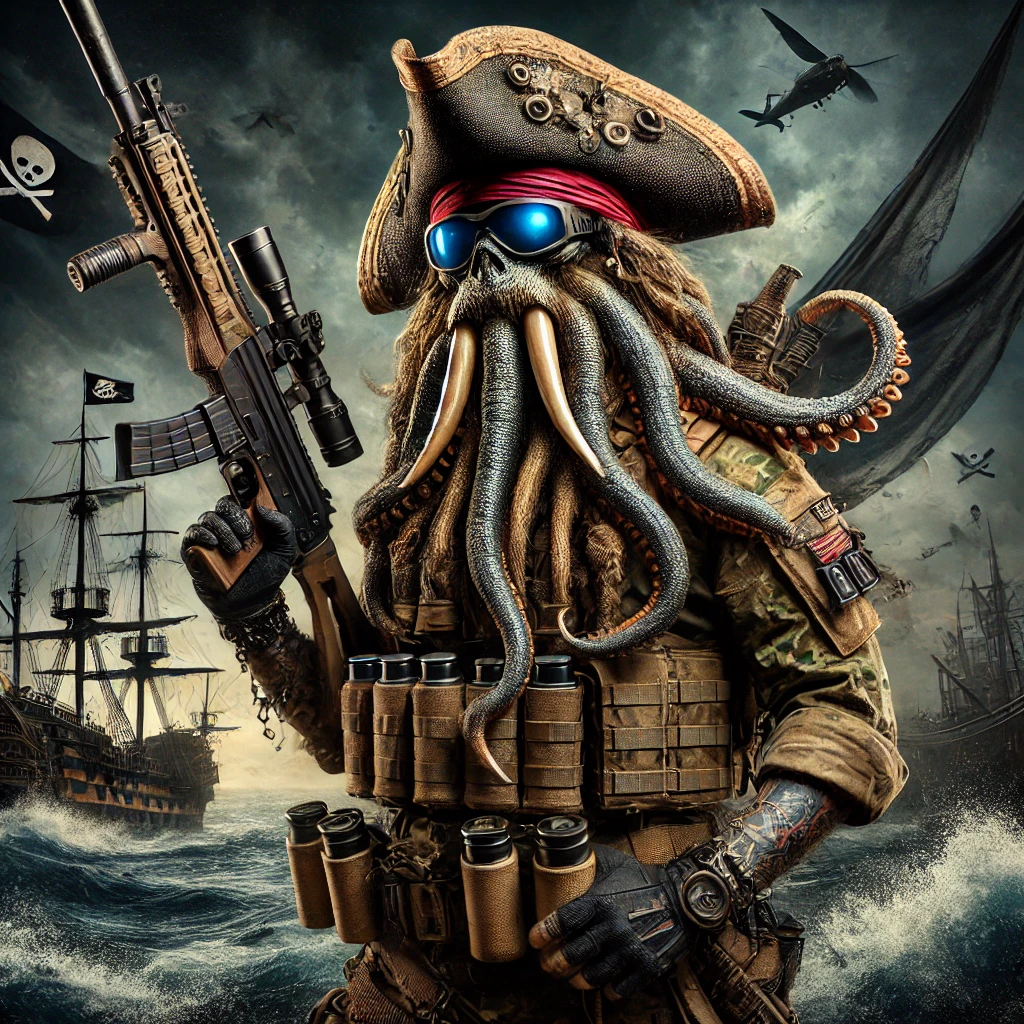
\includegraphics[width=\linewidth]{img/davy-jones.png} % Remplacez 'example-image' par votre image
\end{minipage}
\hfill
\begin{minipage}[t]{0.7\textwidth}
  \begin{itemize}[series=extension]
      \item \textbf{Cartes au trésor :} Des indices pour trouver des caches secrètes.
      \item \textbf{Leurres :} Faux trésors ou pièges pour détourner les adversaires.
      \item \textbf{PNJ - Davy Jones :} Un adversaire redoutable qui protège un trésor précieux.
      \item \textbf{Quêtes spéciales :} Prendre le contrôle d’une forteresse et la tenir pendant 5 minutes pour obtenir un trésor inestimable.
      \item \textbf{Trésors temporaires :} Des trésors cachés dans une zone dangereuse, disponibles seulement pour un temps limité.
  \end{itemize}
\end{minipage}
\begin{itemize}[resume*=extension]
    \item \textbf{Le Masque du Roi maudit :} Ajoutez un masque en or maudit, symbole d'une ancienne malédiction. Le pirate portant ce trésor est condamné à signaler sa position toutes les 10 secondes en criant "MAUDIT", attirant ainsi les convoitises de ses ennemis.
    \item \textbf{Le Coffre du Kraken :} Un immense coffre renfermant un trésor d'une valeur inestimable. Tellement imposant qu'il nécessite deux pirates pour le transporter. Ces derniers, accaparés par le poids du coffre, ne pourront pas utiliser leurs répliques, rendant leur progression périlleuse.
    \item \textbf{Les porteurs désignés :} Chaque équipage doit choisir, avant de lever l’ancre, les deux seuls pirates autorisés à transporter les trésors. Ce privilège sacré les transforme en cibles de choix pour l’équipage adverse !
    \item \textbf{Trésors de quête :} Les trésors gagnés lors des quêtes peuvent être des butins classiques ou des reliques inviolables, réservées à l’équipage ayant accompli l’exploit. Ces trésors deviennent un symbole de leur bravoure !
\end{itemize}


\vspace{2cm}

\begin{center}
  {\Huge Amusez vous et prenez du plaisir} \\
  \vspace{1.5cm}
  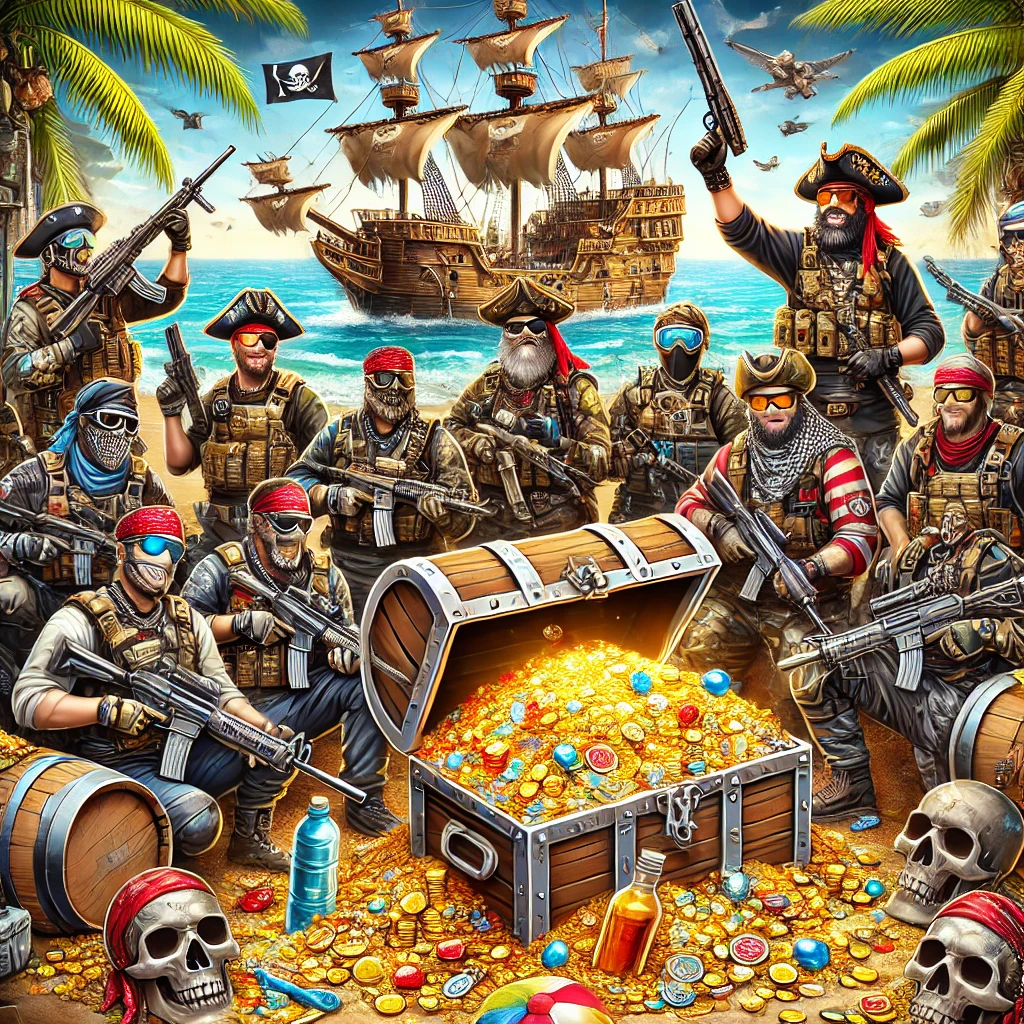
\includegraphics[width=0.6\linewidth]{img/end.png} \\
  \vspace{1cm}
  Scénario créé par :\\
  Jérémy
\end{center}

\newpage

\section*{Fiche d'aide - Calcul des points}

\begin{center}
  \renewcommand{\arraystretch}{1.5}
  \begin{tabular}{|p{3cm}|p{2cm}|p{2cm}|p{2cm}|p{2cm}|p{2cm}|}
    \hline
    \multicolumn{2}{|c|}{\textbf{Trésor}} & \multicolumn{2}{c|}{\textbf{Équipe 1}} & \multicolumn{2}{c|}{\textbf{Équipe 2}} \\ \hline
    \textbf{Type de trésor} & \textbf{Valeur} & \textbf{Nombre trouvé} & \textbf{Total} & \textbf{Nombre trouvé} & \textbf{Total} \\ \hline
    Pièces                 &                 &                         &                &                         &                \\ \hline
    Gemmes                 &                 &                         &                &                         &                \\ \hline
    Statuette              &                 &                         &                &                         &                \\ \hline
    Masque                 &                 &                         &                &                         &                \\ \hline
    ...                  &                 &                         &                &                         &                \\ \hline
    ...                  &                 &                         &                &                         &                \\ \hline
    ...                  &                 &                         &                &                         &                \\ \hline
    \multicolumn{2}{|c|}{\textbf{Total}}    &                         &                &                         &                \\ \hline
  \end{tabular}
  \bigskip

  \begin{tabular}{|p{3cm}|p{2cm}|p{2cm}|p{2cm}|p{2cm}|p{2cm}|}
    \hline
    \multicolumn{2}{|c|}{\textbf{Trésor}} & \multicolumn{2}{c|}{\textbf{Équipe 1}} & \multicolumn{2}{c|}{\textbf{Équipe 2}} \\ \hline
    \textbf{Type de trésor} & \textbf{Valeur} & \textbf{Nombre trouvé} & \textbf{Total} & \textbf{Nombre trouvé} & \textbf{Total} \\ \hline
    Pièces                 &                 &                         &                &                         &                \\ \hline
    Gemmes                 &                 &                         &                &                         &                \\ \hline
    Statuette              &                 &                         &                &                         &                \\ \hline
    Masque                 &                 &                         &                &                         &                \\ \hline
    ...                  &                 &                         &                &                         &                \\ \hline
    ...                  &                 &                         &                &                         &                \\ \hline
    ...                  &                 &                         &                &                         &                \\ \hline
    \multicolumn{2}{|c|}{\textbf{Total}}    &                         &                &                         &                \\ \hline
  \end{tabular}
  \bigskip

  \begin{tabular}{|p{3cm}|p{2cm}|p{2cm}|p{2cm}|p{2cm}|p{2cm}|}
    \hline
    \multicolumn{2}{|c|}{\textbf{Trésor}} & \multicolumn{2}{c|}{\textbf{Équipe 1}} & \multicolumn{2}{c|}{\textbf{Équipe 2}} \\ \hline
    \textbf{Type de trésor} & \textbf{Valeur} & \textbf{Nombre trouvé} & \textbf{Total} & \textbf{Nombre trouvé} & \textbf{Total} \\ \hline
    Pièces                 &                 &                         &                &                         &                \\ \hline
    Gemmes                 &                 &                         &                &                         &                \\ \hline
    Statuette              &                 &                         &                &                         &                \\ \hline
    Masque                 &                 &                         &                &                         &                \\ \hline
    ...                  &                 &                         &                &                         &                \\ \hline
    ...                  &                 &                         &                &                         &                \\ \hline
    ...                  &                 &                         &                &                         &                \\ \hline
    \multicolumn{2}{|c|}{\textbf{Total}}    &                         &                &                         &                \\ \hline
  \end{tabular}
\end{center}

\newpage

\section*{Fiche d'aide - Calcul du nombre de trésors}

\input{repartition.tex}

\end{document}
